\documentclass[12pt]{article}
\usepackage{../../ficha}

\begin{document}

\ficha{Histogramas, Quartis e Diagramas de Extremos e Quartis}

\instrucoes{Resolve os exercícios, apresentando os cálculos. Para determinar os quartis, ordena primeiro os dados.}

\secao{Dados Agrupados em Classes}{As alturas, em cm, de 20 alunos de uma turma são as seguintes.}

\begin{center}
\begin{tabular}{cccccccccc}
  152 & 158 & 161 & 147 & 165 & 170 & 155 & 149 & 162 & 168 \\
  159 & 151 & 163 & 157 & 166 & 172 & 154 & 160 & 156 & 164 \\
\end{tabular}
\end{center}

\begin{exercicios}
  \item Completa a tabela de frequências com as classes $[145, 150[$, $[150, 155[$, $[155, 160[$, $[160, 165[$, $[165, 170[$ e $[170, 175[$.
  \item Qual é a amplitude de cada classe?
  \item Qual é a classe modal?
  \item Que percentagem de alunos tem pelo menos 160\,cm?
  \item Constrói o histograma correspondente.
  \item Constrói o polígono de frequências.
\end{exercicios}

\secao{Interpretação de Histogramas}{O histograma representa os tempos, em minutos, que os alunos de uma escola demoram a chegar à escola.}

\begin{center}
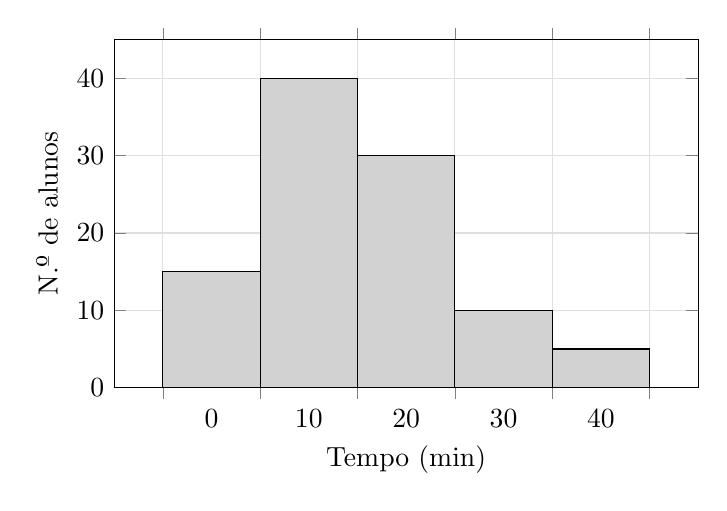
\begin{tikzpicture}
\begin{axis}[ybar interval, ymin=0, ymax=45, xtick={0,10,20,30,40,50}, ytick={0,10,...,40}, xlabel={Tempo (min)}, ylabel={N.º de alunos}, width=9cm, height=6cm, grid=major, grid style={gray!25}]
  \addplot[fill=gray!35] coordinates {(0,15) (10,40) (20,30) (30,10) (40,5) (50,0)};
\end{axis}
\end{tikzpicture}
\end{center}

\begin{exercicios}
  \item Quantos alunos foram inquiridos?
  \item Quantos alunos demoram menos de 20 minutos?
  \item Que percentagem de alunos demora 30 minutos ou mais?
  \item Qual é a classe modal?
  \item Em que classe está a mediana? Justifica.
  \item Estima a média usando os pontos médios das classes.
\end{exercicios}

\secao{Diagramas de Caule-e-Folhas}{Os pontos marcados por uma equipa de basquetebol em 15 jogos estão no diagrama de caule-e-folhas.}

\begin{center}
\begin{tabular}{r|l}
  5 & 2\; 8 \\
  6 & 1\; 4\; 4\; 7 \\
  7 & 0\; 3\; 5\; 5\; 9 \\
  8 & 2\; 6\; 8 \\
  9 & 1 \\
\end{tabular}
\qquad \small Legenda: $5\,|\,2$ significa 52 pontos.
\end{center}

\begin{exercicios}
  \item Qual foi a maior e a menor pontuação? Calcula a amplitude.
  \item Qual é a moda?
  \item Qual é a mediana?
  \item Em quantos jogos a equipa marcou 70 ou mais pontos?
  \item Calcula a média dos pontos (arredonda às décimas).
\end{exercicios}

\secao{Quartis e Amplitude Interquartis}{Para cada conjunto de dados, determina o mínimo, o 1.º quartil, a mediana, o 3.º quartil, o máximo e a amplitude interquartis.}
\begin{exercicios}
  \item $3,\ 5,\ 7,\ 8,\ 9,\ 11,\ 13$
  \item $2,\ 4,\ 4,\ 6,\ 8,\ 9,\ 10,\ 12$
  \item $15,\ 22,\ 18,\ 30,\ 25,\ 20,\ 27,\ 19,\ 24$
  \item $1{,}2;\ 3{,}4;\ 2{,}8;\ 4{,}1;\ 3{,}0;\ 2{,}5;\ 3{,}9;\ 1{,}8;\ 2{,}2;\ 3{,}6$
  \item As classificações de um teste: $45,\ 52,\ 60,\ 61,\ 68,\ 70,\ 72,\ 75,\ 80,\ 85,\ 88,\ 95$.
  \item O que representa, em percentagem, o intervalo entre o 1.º e o 3.º quartil?
\end{exercicios}

\secao{Diagramas de Extremos e Quartis}{Observa os diagramas, que representam as classificações (0 a 100) de duas turmas num teste.}

\begin{center}
\begin{tikzpicture}[x=0.11cm]
  \draw[-{Latex}] (0,0) -- (105,0);
  \foreach \i in {0,10,...,100} {\draw (\i,0.1) -- (\i,-0.1); \node[below, font=\footnotesize] at (\i,-0.1) {\i};}
  % Turma A: 30, 50, 62, 75, 95
  \begin{scope}[yshift=1.2cm]
    \node[left] at (-2,0) {A};
    \draw (30,0) -- (50,0); \draw (75,0) -- (95,0);
    \draw (50,-0.3) rectangle (75,0.3); \draw (62,-0.3) -- (62,0.3);
    \draw (30,-0.2) -- (30,0.2); \draw (95,-0.2) -- (95,0.2);
  \end{scope}
  % Turma B: 40, 55, 65, 70, 85
  \begin{scope}[yshift=2.4cm]
    \node[left] at (-2,0) {B};
    \draw (40,0) -- (55,0); \draw (70,0) -- (85,0);
    \draw (55,-0.3) rectangle (70,0.3); \draw (65,-0.3) -- (65,0.3);
    \draw (40,-0.2) -- (40,0.2); \draw (85,-0.2) -- (85,0.2);
  \end{scope}
\end{tikzpicture}
\end{center}

\begin{exercicios}
  \item Indica os cinco números-resumo (mínimo, $Q_1$, mediana, $Q_3$, máximo) de cada turma.
  \item Qual das turmas tem maior amplitude? E maior amplitude interquartis?
  \item Em que turma é que pelo menos metade dos alunos teve 65 ou mais?
  \item Na turma A, que percentagem de alunos teve classificação entre 50 e 75?
  \item Qual das turmas tem resultados mais homogéneos? Justifica.
  \item Constrói o diagrama de extremos e quartis dos dados do exercício 5 da secção anterior.
\end{exercicios}

\secao{Desafios}{Resolve os problemas.}
\begin{exercicios}
  \item Escreve um conjunto de 7 dados com mínimo 2, máximo 20, mediana 10 e $Q_1 = 5$.
  \item Num conjunto de dados, $Q_1 = 12$ e $Q_3 = 30$. Um valor é considerado atípico se for maior do que $Q_3 + 1{,}5 \times (Q_3 - Q_1)$. A partir de que valor um dado é atípico?
  \item Acrescentando o valor 100 aos dados $3, 5, 7, 8, 9, 11, 13$, o que acontece à média? E à mediana? Qual das medidas é mais afetada?
  \item Dois conjuntos de dados têm a mesma mediana mas amplitudes interquartis muito diferentes. O que se pode concluir?
\end{exercicios}

\end{document}
